\chapter{Ansteuerung eines RDC}
\label{ch:micbac}


\begin{figure}[H]
	\begin{minipage}{0.5\textwidth}
		\centering
		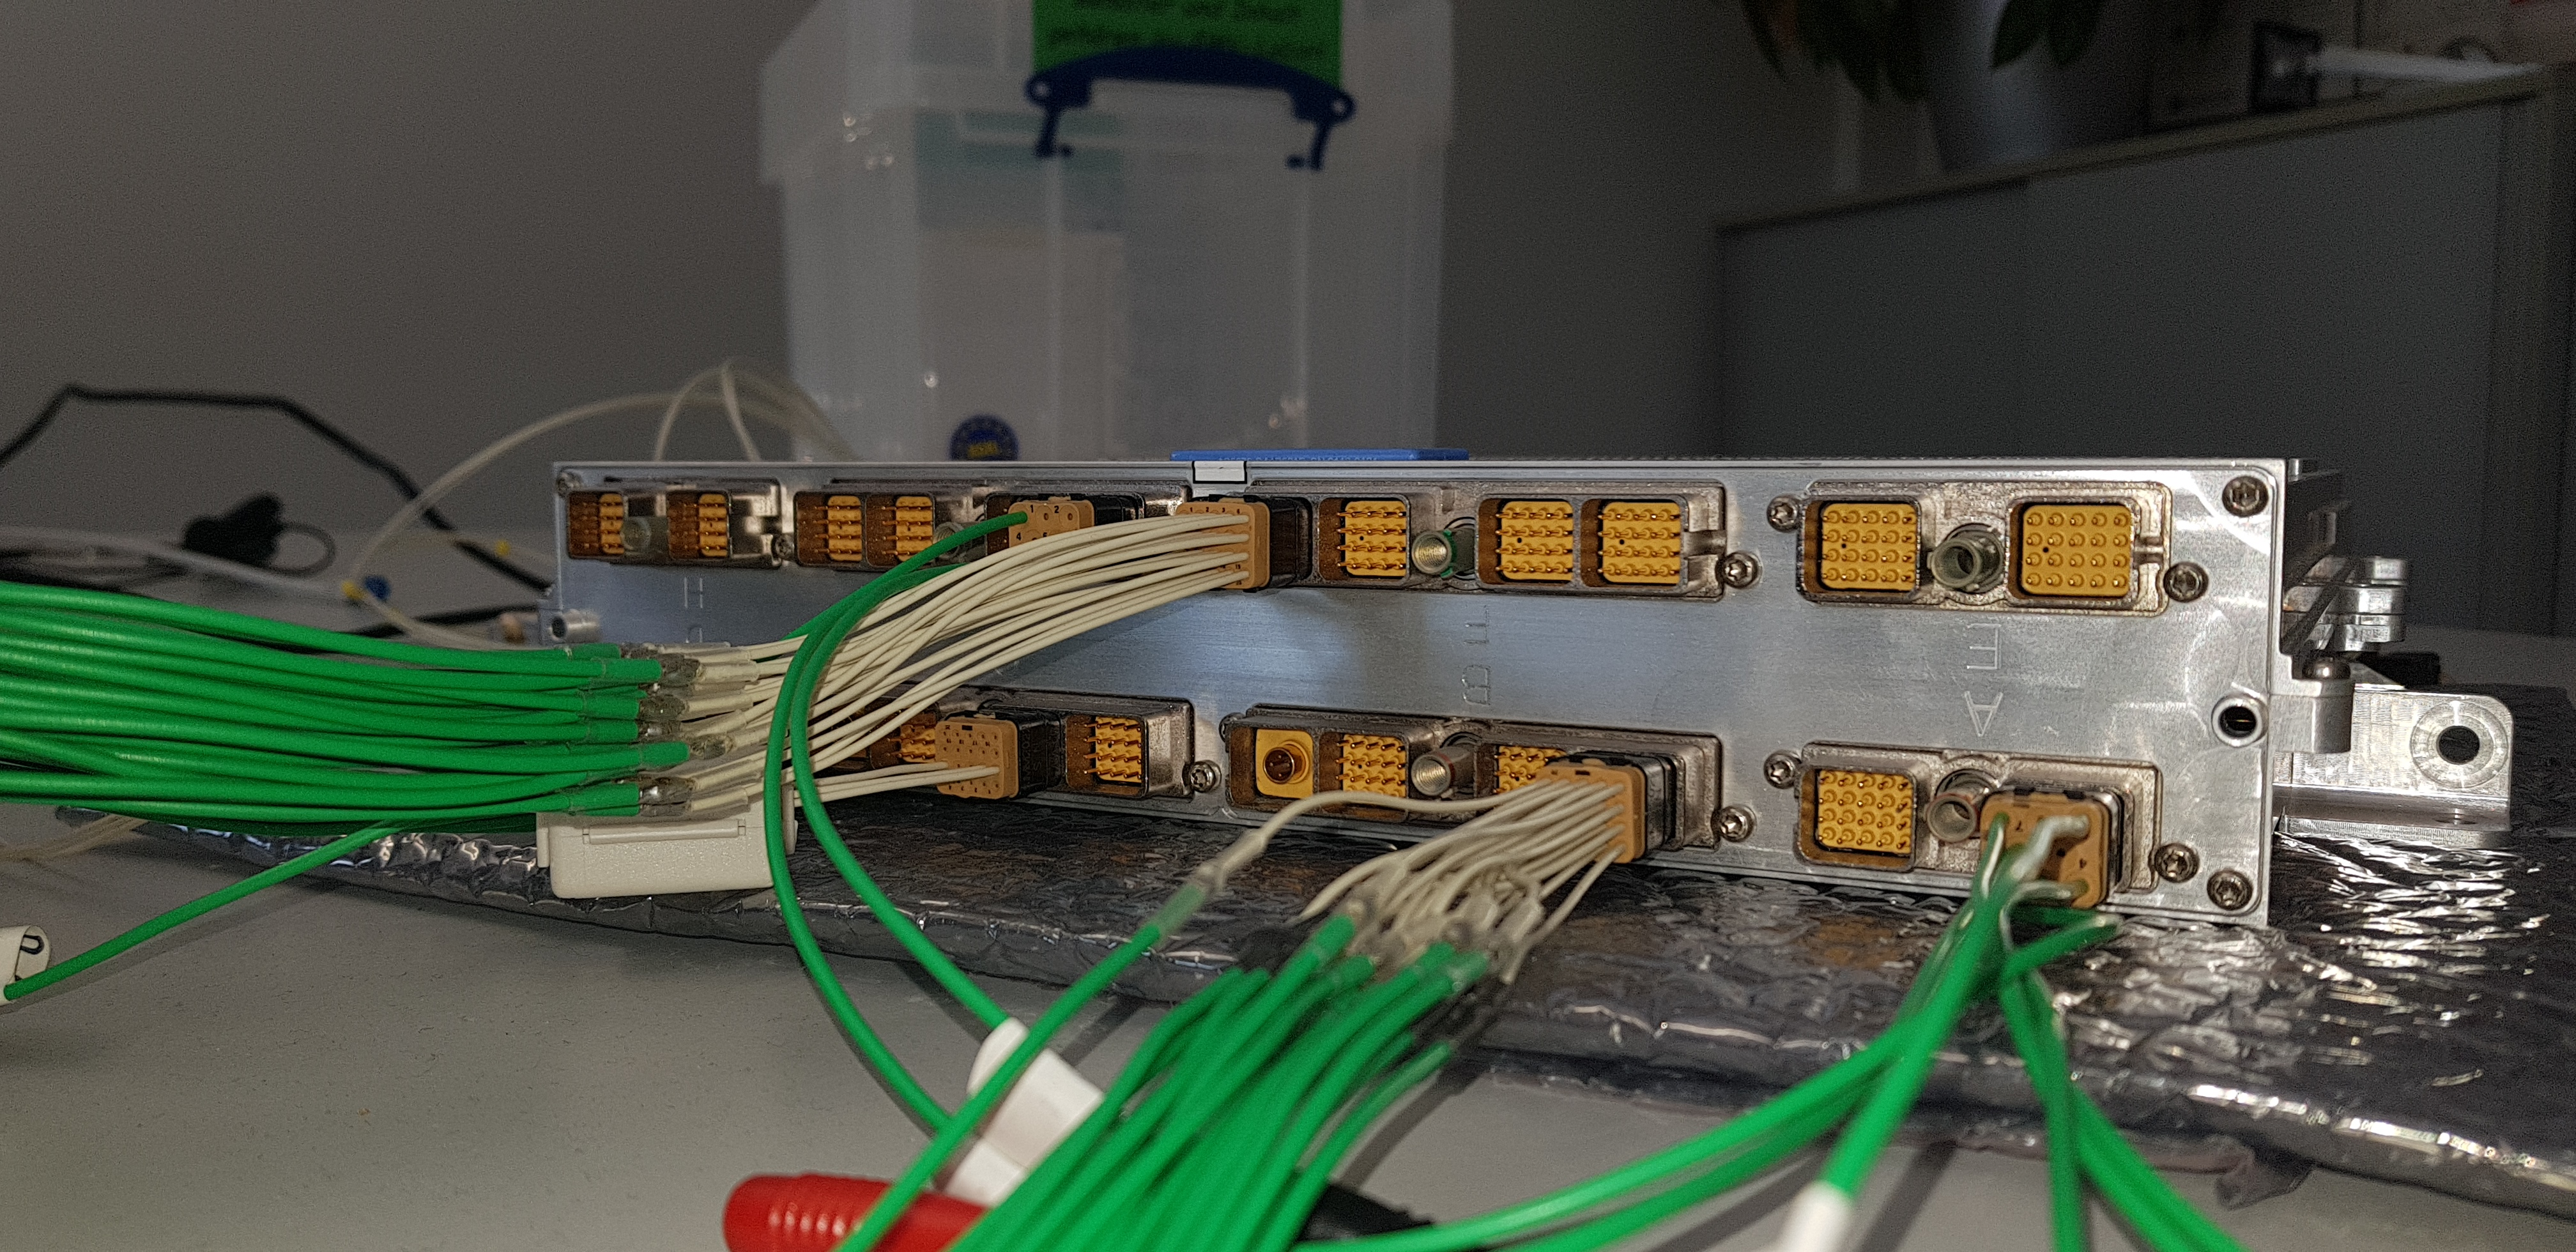
\includegraphics[width=\textwidth, height=0.5\textwidth]{graphics/crdc_1.png}
		\caption{CRDC Type A Pins}
		\label{fig:crdc-pins}
	\end{minipage}
	\begin{minipage}{0.5\textwidth}
		\centering
		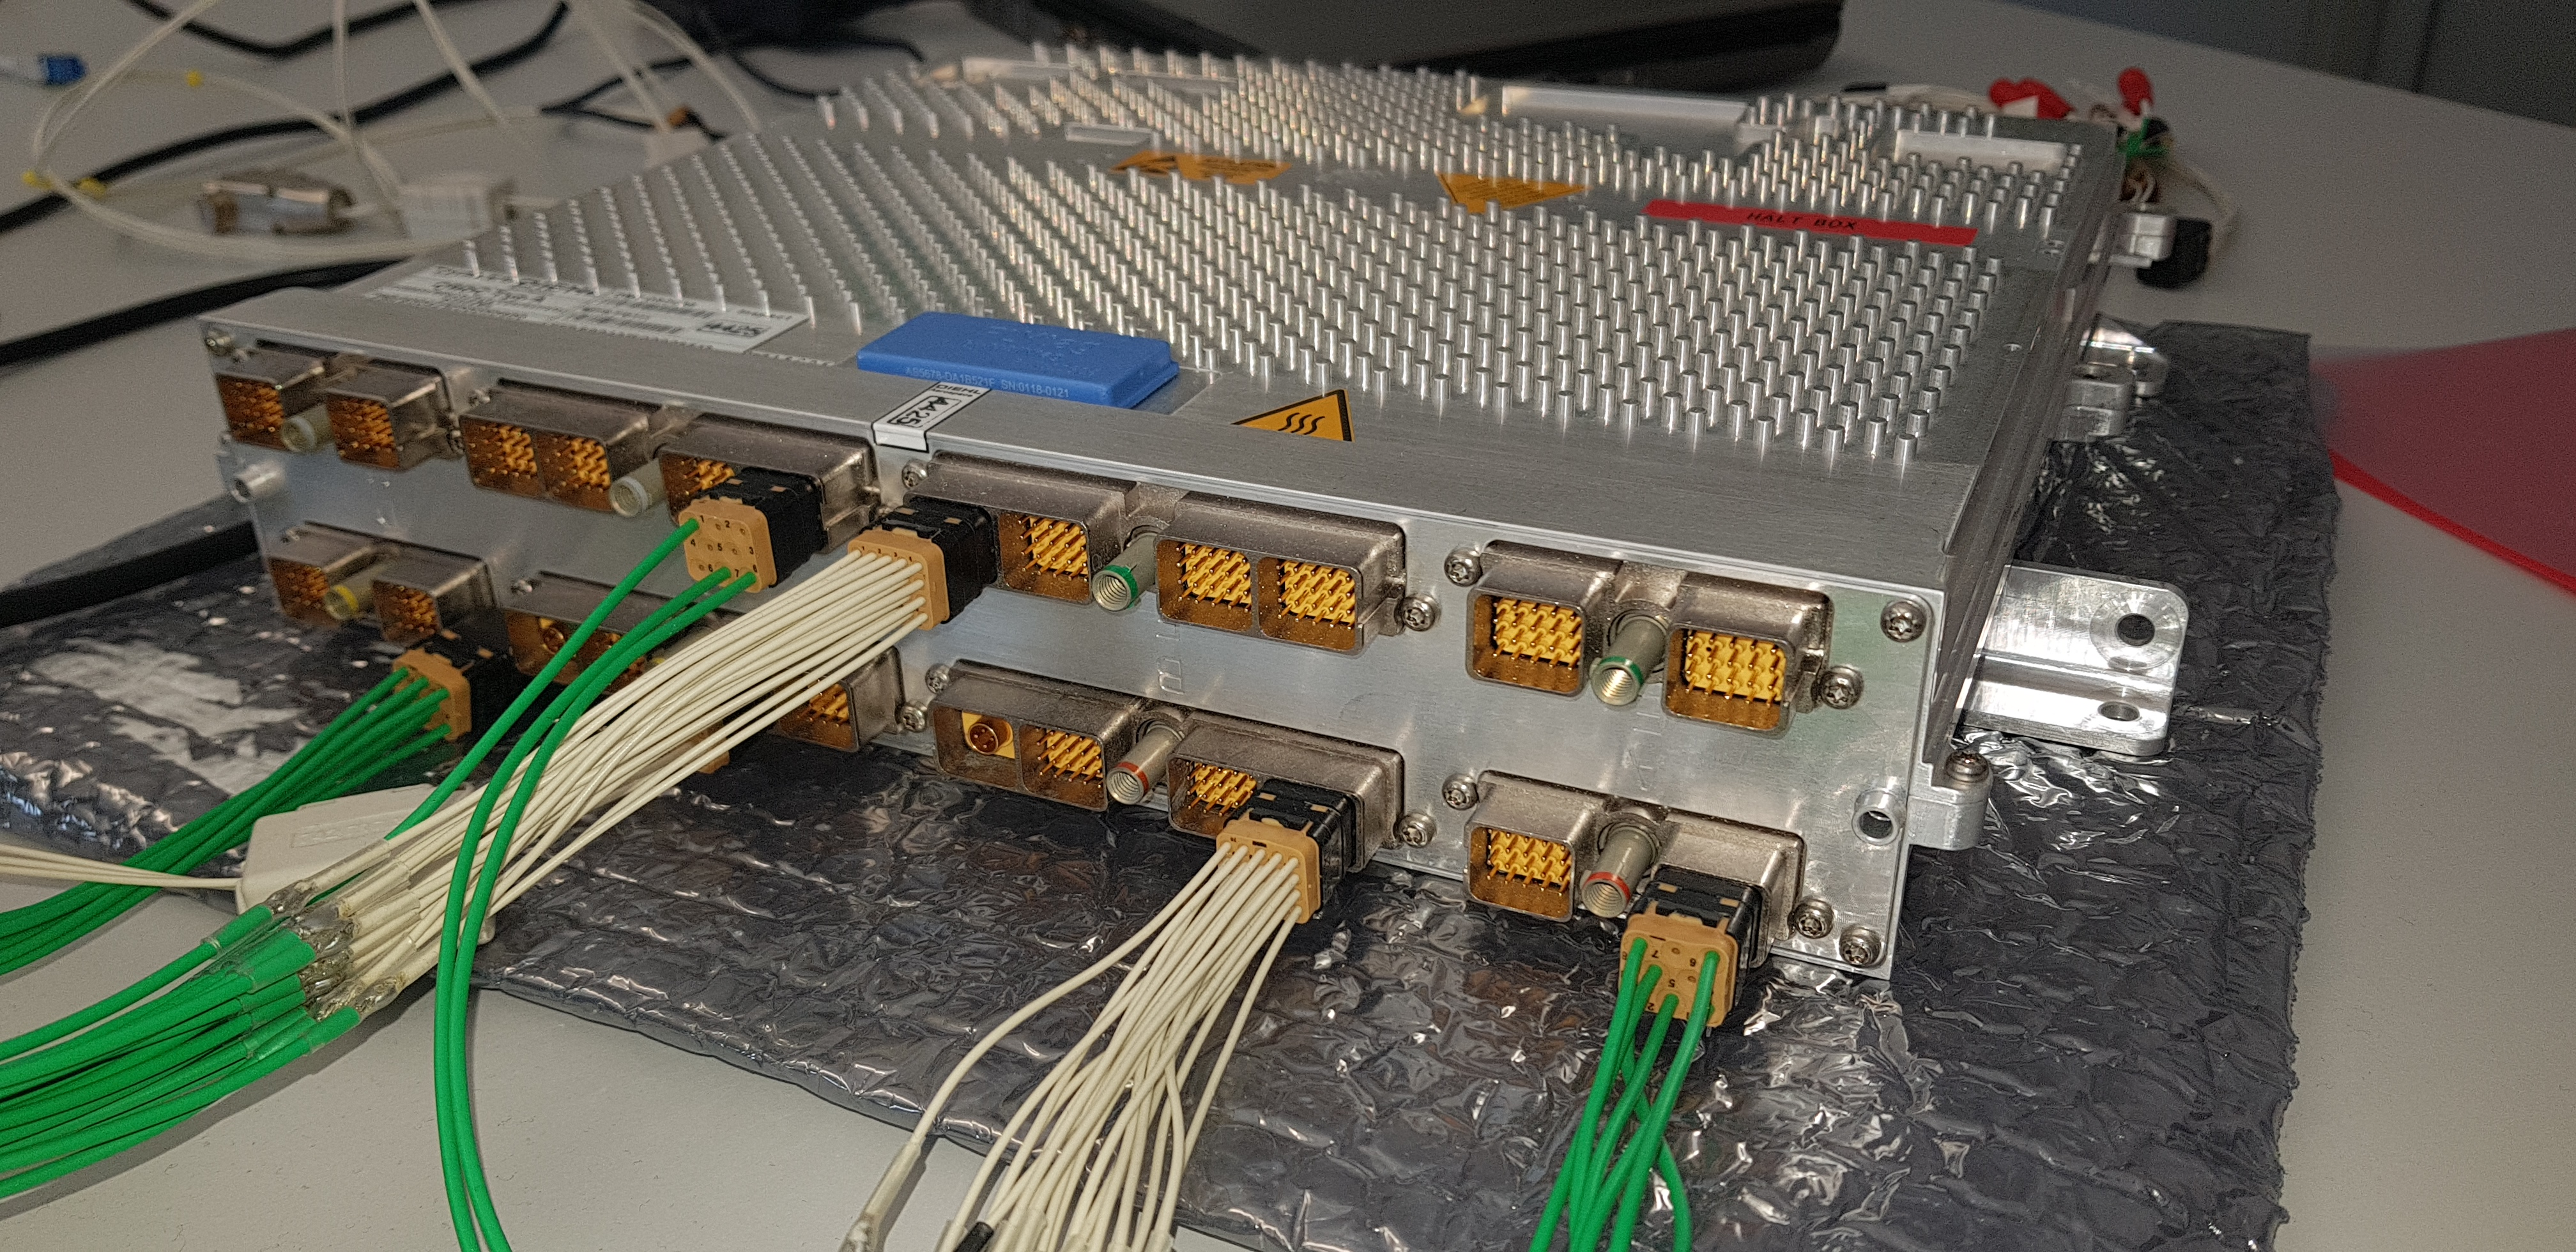
\includegraphics[width=\textwidth, height=0.5\textwidth]{graphics/crdc_2.png}
		\caption{CRDC Type A}
		\label{fig:crdc_top}
	\end{minipage}
\end{figure}



footnote und etc

\section{Verbindung herstellen über das RS232-Interface}
\label{sec:rs232-connection}

mach sachen

\section{Befehle Senden und Empfangen}
\label{sec:com-send-receive}

\subsection{MICBAC Commands}
\label{subsec:micbac-commands}

\subsection{Senden von MICBAC Commands}
\label{subsec:send-micbac}


\inputpython{scripts/send_micbac.py}{1}{15}{Send MICBAC Command}{lst:send-micbac}

\subsection{Empfangen von MICBAC Commands}
\label{subsec:receive-micbac}

\inputpython{scripts/receive_micbac.py}{1}{9}{Receive MICBAC Command}{lst:receive-micbac}